%%%%%%%%%%%%%%%%%%%%%%%%%%%%%%%%%%%%%%%%%%%%%%%%%%%%%
%												    %
%	LCOM PROJECT PROPOSAL				    		%
%												    %
%	Novembro 2015								    %
%												    %
%	Angela Cardodo and Ilona Generalova				%
%   											    %	
%%%%%%%%%%%%%%%%%%%%%%%%%%%%%%%%%%%%%%%%%%%%%%%%%%%%%

\documentclass[11pt,a4paper,reqno]{report}
\linespread{1.2}


\usepackage{rotating}
\usepackage{tikz}
\usepackage[active]{srcltx}    
\usepackage{graphicx}
\usepackage{amsthm,amsfonts,amsmath,amssymb,indentfirst,mathrsfs,amscd}
\usepackage[mathscr]{eucal}
\usepackage{tensor}
\usepackage[utf8x]{inputenc}
%\usepackage[portuges]{babel}
\usepackage[T1]{fontenc}
\usepackage{enumitem}
\setlist{nolistsep}
\usepackage{comment} 
\usepackage{tikz}
\usepackage[numbers,square, comma, sort&compress]{natbib}
\usepackage[nottoc,numbib]{tocbibind}
%\numberwithin{figure}{section}
\numberwithin{equation}{section}
\usepackage{scalefnt}
\usepackage[top=2cm, bottom=2cm, left=2cm, right=2cm]{geometry}
\usepackage{MnSymbol}
%\usepackage[pdfpagelabels,pagebackref,hypertexnames=true,plainpages=false,naturalnames]{hyperref}
\usepackage[naturalnames]{hyperref}
\usepackage{enumitem}
\usepackage{titling}
\newcommand{\subtitle}[1]{%
	\posttitle{%
	\par\end{center}
	\begin{center}\large#1\end{center}
	\vskip0.5em}%
}
\newcommand{\HRule}{\rule{\linewidth}{0.5mm}}
\usepackage{caption}
\usepackage{etoolbox}% http://ctan.org/pkg/etoolbox
\usepackage{complexity}

\usepackage[official]{eurosym}

\def\Cpp{C\raisebox{0.5ex}{\tiny\textbf{++}}}

\makeatletter
\def\@makechapterhead#1{%
  \vspace*{2\p@}%
  {\parindent \z@ \raggedright \normalfont
    \ifnum \c@secnumdepth >\m@ne
%        \huge\bfseries \@chapapp\space \thechapter
        \par\nobreak
        \vskip 4\p@
    \fi
    \interlinepenalty\@M
    \Huge \bfseries \thechapter\space #1\par\nobreak
    \vskip 10\p@
  }}
\def\@makeschapterhead#1{%
  \vspace*{2\p@}%
  {\parindent \z@ \raggedright
    \normalfont
    \interlinepenalty\@M
    \Huge \bfseries  #1\par\nobreak
%    \vskip 5\p@
  }}
\makeatother

\usepackage[toc,page]{appendix}


%\addto\captionsportuges{%
%  \renewcommand\appendixname{Anexo}
%  \renewcommand\appendixpagename{Anexos}
%  \renewcommand\appendixtocname{Anexos}
%  \renewcommand\abstractname{\huge Sumário}  
%}

\usepackage{verbatim}
\usepackage{color}
\definecolor{darkgray}{rgb}{0.41, 0.41, 0.41}
\definecolor{green}{rgb}{0.0, 0.5, 0.0}
\usepackage{listings}
\lstset{language=C++, 
	numbers=left,
	firstnumber=1,
	numberfirstline=true,
    basicstyle=\linespread{0.8}\ttfamily,
    keywordstyle=\color{blue}\ttfamily,
	showstringspaces=false,
    stringstyle=\color{red}\ttfamily,
    commentstyle=\color{green}\ttfamily,
	identifierstyle=\color{darkgray}\ttfamily,
    morecomment=[l][\color{magenta}]{\#},
	tabsize=4,
    breaklines=true
}

\begin{document}



\begin{titlepage}
\begin{center}
 
\vspace*{3cm}

{\Large Computer Laboratory}\\[2cm]

% Title
{\Huge \bfseries Project Proposal \\[1cm]}

% Author
{\large \^Angela Cardoso and Ilona Generalova}\\[2cm]


\includegraphics[width=10cm]{feup_logo.jpg}\\[2cm]


% Bottom of the page
{\large \today}

\end{center}
\end{titlepage}


%%%%%%%%%%%
% SUMARIO %
%%%%%%%%%%%
\begin{abstract}
	
As the final project for the course of Computer Laboratory at FEUP, we decided to develop a Minix version of the card game Set. We tried to use all the devices, and with the exception of the serial port where able to do so. This document presents the description of the game and its implementation, with focus on the devices used and their role, the modules developed and some implementation details.

\end{abstract}

\tableofcontents

%%%%%%%%%%%%%%
% INSTRUCOES %
%%%%%%%%%%%%%%
\chapter{User instructions}

\section{The game Set}

Since Set is not a wildly known game, we need to start with explaining it, before diving into the application we built to play it.
2
Set is a card game that should be played in real time, in the sense that all players may act simultaneously. It was designed by Marsha Falco in 1974. There are 81 cards in a deck of Set, they are all distinct and have 4 varying features:
\begin{itemize}
\item color - red, green or blue;
\item symbol - diamond, oval or squiggle;
\item number - one, two or three;
\item shading - open, stripped or solid.
\end{itemize}
Each card has one of the possible combinations of these features, for example, there is a card with three striped green diamonds, and another card with one solid blue squiggle.

There are several games that can be played with these cards, but they all involve the concept of a set. A set consists of three cards such that for each feature, they all agree or they all differ. That is:
\begin{itemize}
\item they all have the same color or they all have different colors;
\item they all have the same symbol or they all have different symbols;
\item they all have the same number or they all have different numbers;
\item they all have the same shading or they all have different shadings.
\end{itemize}
For example, these three cards, shown in Figure~\ref{set} form a set:
\begin{itemize}
\item one green open diamond;
\item two blue stripped squiggles;
\item three red solid ovals.
\end{itemize}
This implies that given any two cards from the deck, there will be exactly one other card that forms a set with them.

\begin{figure}[htbp]
\begin{center}
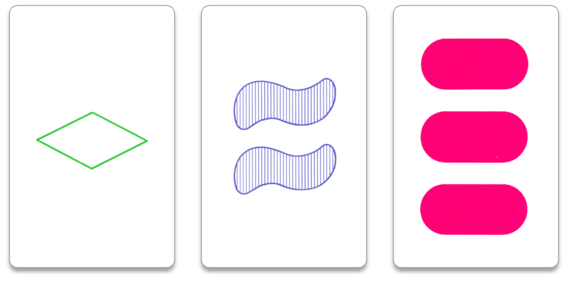
\includegraphics[scale=0.4]{set.png}
\caption{Example of a Set.}
\label{set}
\end{center}
\end{figure}

In the standard Set game, twelve cards are laid down. The first player that sees a set calls ``Set!'' and takes the cards in the set. Three new cards are dealt to replace those and the game proceeds. If a player makes a mistake and chooses three cards that do not form a set, they are penalized. If there is no set among the twelve cards, the dealer deals out three more cards to make fifteen dealt cards, or eighteen or more, as necessary. This process of dealing by threes and finding sets continues until the deck is exhausted and there are no more sets on the table. At this point, whoever has collected the most sets wins.

\section{Game Menus}

\begin{figure}[htbp]
\begin{center}
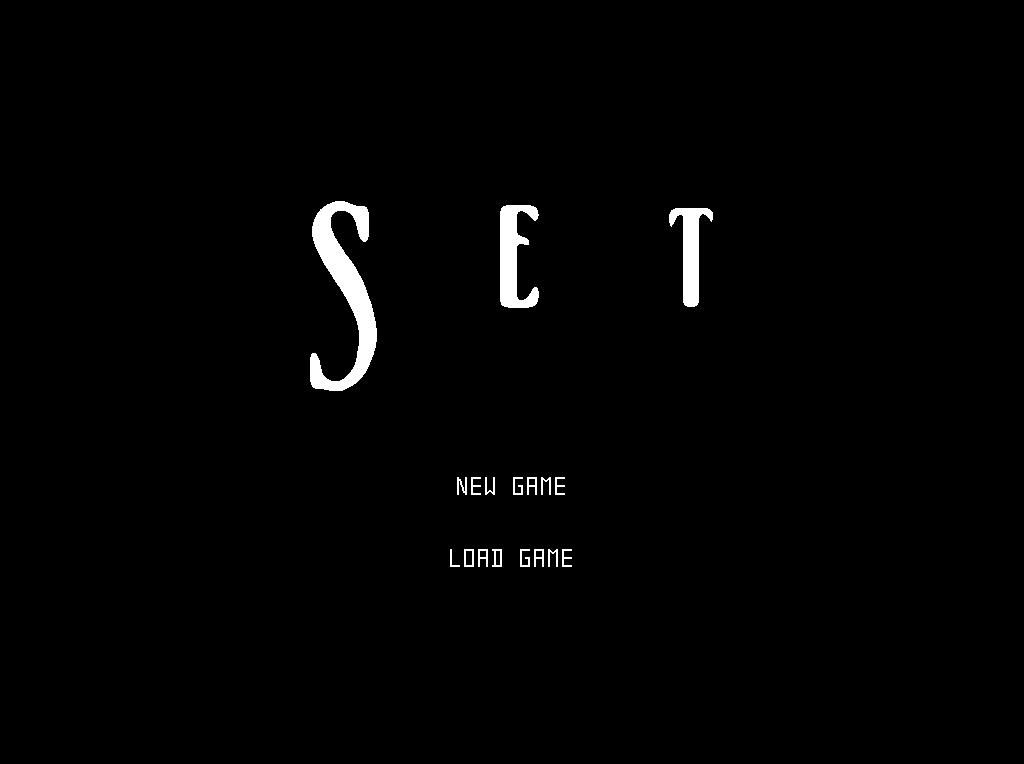
\includegraphics[scale=0.3]{menu_init.png}
\caption{Initial game menu.}
\label{menu_init}
\end{center}
\end{figure}

Upon start, the game presents us its initial menu, shown in Figure~\ref{menu_init}, where the player may choose between starting a new game or loading a previously saved game. This choice is done using the mouse to click on the desired text.

\begin{figure}[htbp]
\begin{center}
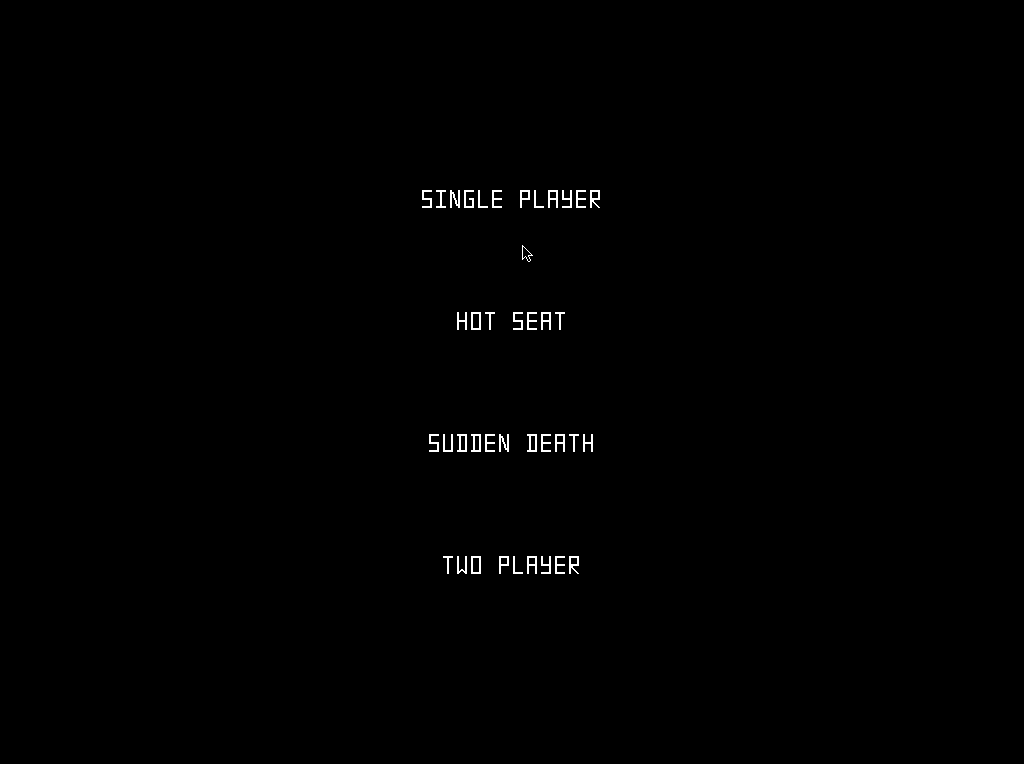
\includegraphics[scale=0.3]{menu_new.png}
\caption{New game menu.}
\label{menu_new}
\end{center}
\end{figure}

The option to load a game is not implemented, so clicking on it does nothing. But the menu was actually designed and so where the plans for its implementation. The idea is to provide four slots for loading games, corresponding to four predefined text files that would be generated by the application. There would also be a corresponding save game menu, with the same four game slots.

\begin{figure}[htbp]
\begin{center}
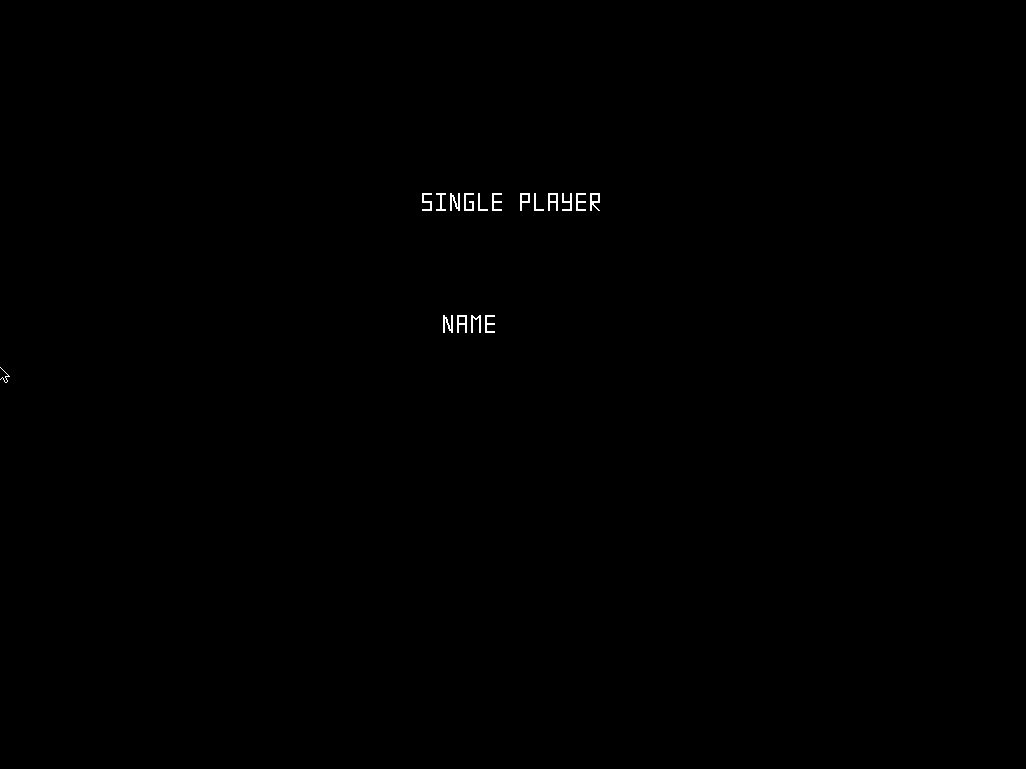
\includegraphics[scale=0.3]{menu_single.png}
\caption{Single player menu.}
\label{menu_single}
\end{center}
\end{figure}

\begin{figure}[htbp]
\begin{center}
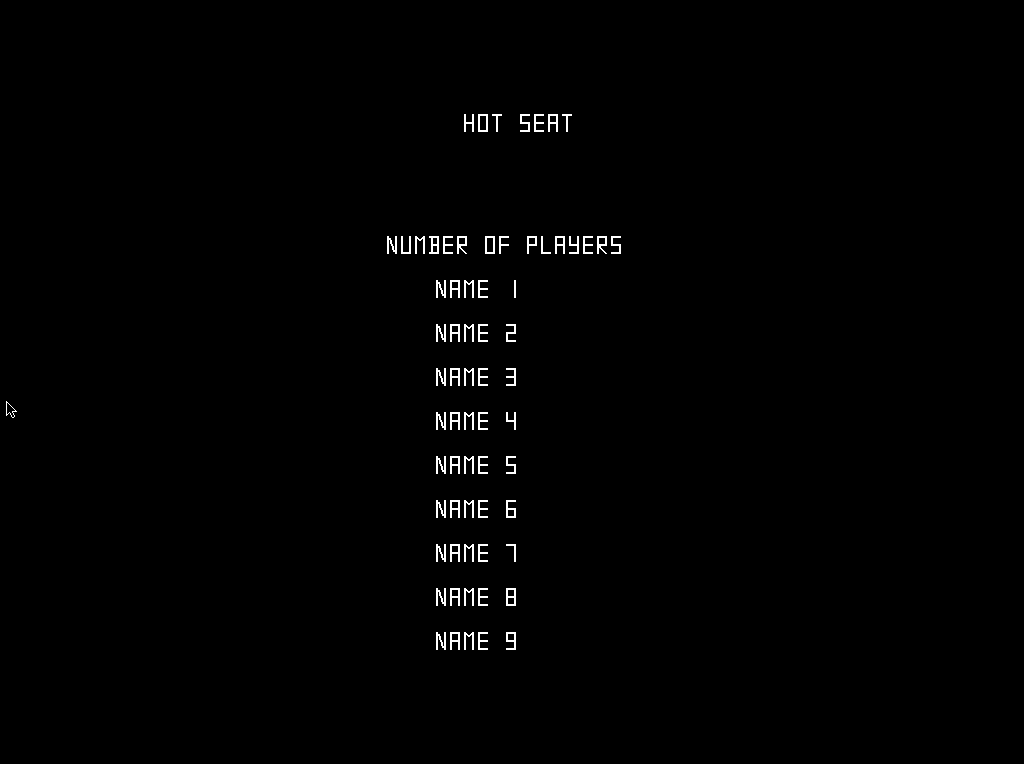
\includegraphics[scale=0.3]{menu_hot.png}
\caption{Hot seat menu.}
\label{menu_hot}
\end{center}
\end{figure}

If the player chooses a new game, a new menu appears as shown in Figure~\ref{menu_new}. There are four types of game to choose from:
\begin{itemize}
\item single player - the player plays alone, trying to obtain the largest possible score by finishing the game fast;
\item hot seat - up to 9 players compete on the same computer to see who gets the largest number of sets;
\item sudden death - the player plays against the clock, having only a limited amount of time to find the next set;
\item two player - two players in two different machines compete to see who gets the most sets.
\end{itemize}

Once again, not all these options have been implemented. Indeed, the first three have menus, and for the last one, the menu was not even implemented. Furthermore, no matter which of the first three game types is chosen, the game play will always be single player. The menus however are built to support the corresponding modes. This means that while the single player and sudden death menus ask only for a single name, see Figure~\ref{menu_single}. The hot seat menu asks for the number of players first and up to nine names, one for each player, as shown in Figure~\ref{menu_hot}.

\begin{figure}[htbp]
\begin{center}
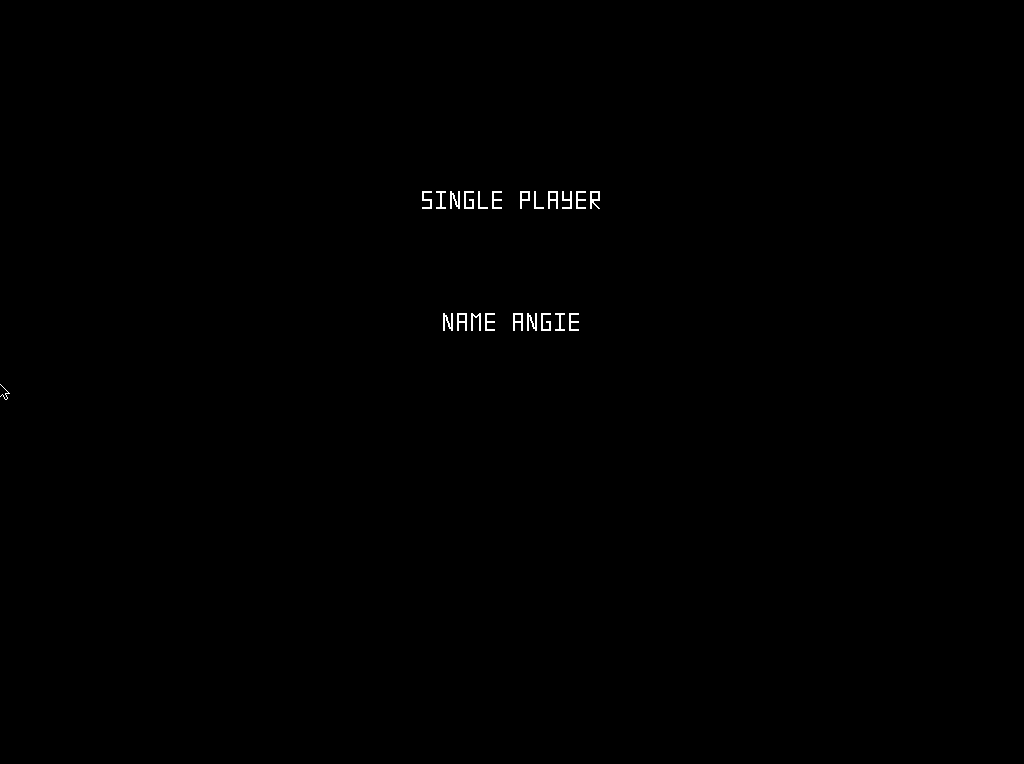
\includegraphics[scale=0.3]{menu_single_name.png}
\caption{Single player menu with name.}
\label{menu_single_name}
\end{center}
\end{figure}

If the user chooses the single player mode, then a name must be entered. This name may have up to five letters, any unused letters will be filled with spaces. The user chooses the name using the keyboard, each letter chosen will be immediately rendered on screen, as shown in Figure~\ref{menu_single_name}. After choosing the name, the user must press the Enter key for the game to actually start. If at any time in the menus the Esc key is pressed, the player is taken back to the initial game menu and must repeat their choices.

\section{Game Play}

\begin{figure}[htbp]
\begin{center}
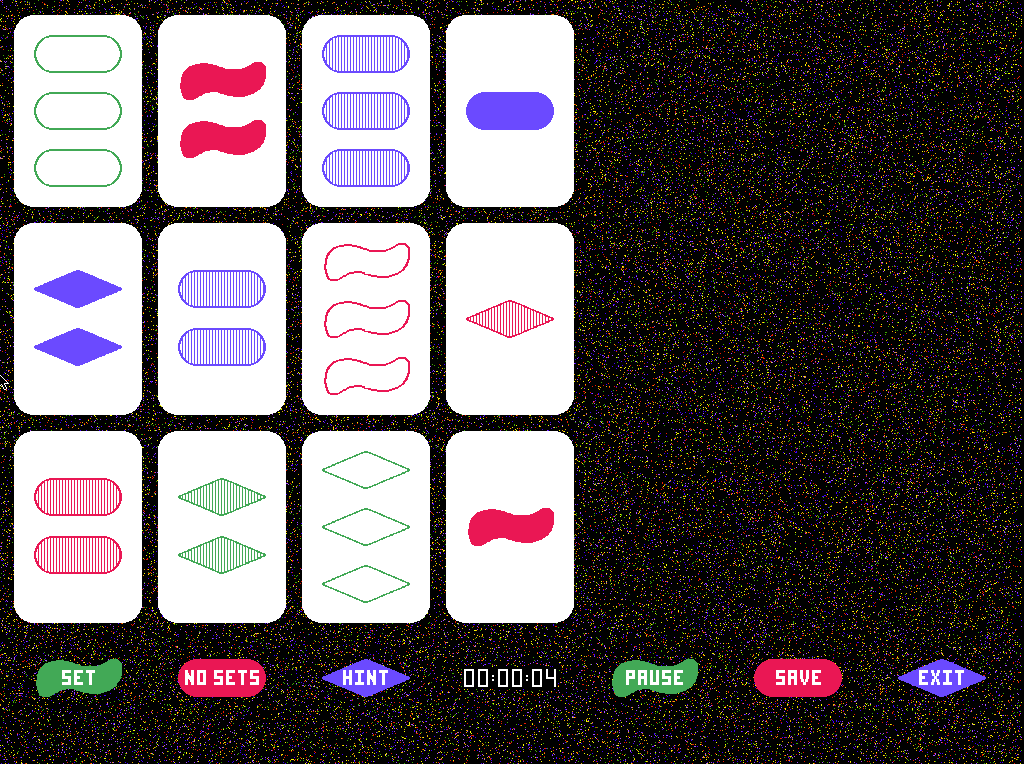
\includegraphics[scale=0.3]{game_play.png}
\caption{A game of Set.}
\label{game_play}
\end{center}
\end{figure}

This leads us to the game screen that can be observed in Figure~\ref{game_play}. The first 12 cards are displayed for the player to find sets among. There are also six buttons and a timer. The timer tells the player how much time as elapsed since the beginning of the game, which is useful since the game time will be used for scoring. The six buttons are:
\begin{itemize}
\item set - after selecting 3 cards that form a set, the player presses this button to remove the set from the game;
\item no sets - if there are no sets among the displayed cards, the player should press this button;
\item hint - if the player wishes to receive a clue, they should press this button;
\item pause - to pause the game, showing the pause screen;
\item save - to save the current game;
\item exit - to leave this game and go back to the initial menu.
\end{itemize}

For each of these buttons there is a corresponding set of keys that may be pressed producing the same effect:
\begin{itemize}
\item set - S or Space keys;
\item no sets - C or Enter keys;
\item hint - H or Shift keys;
\item pause - P or Ctrl keys;
\item save - W or Alt keys;
\item exit - E or Esc keys.
\end{itemize}
Since the game is timed, these keys can be very useful, because they reduce the time of play significantly.

\begin{figure}[htbp]
\begin{center}
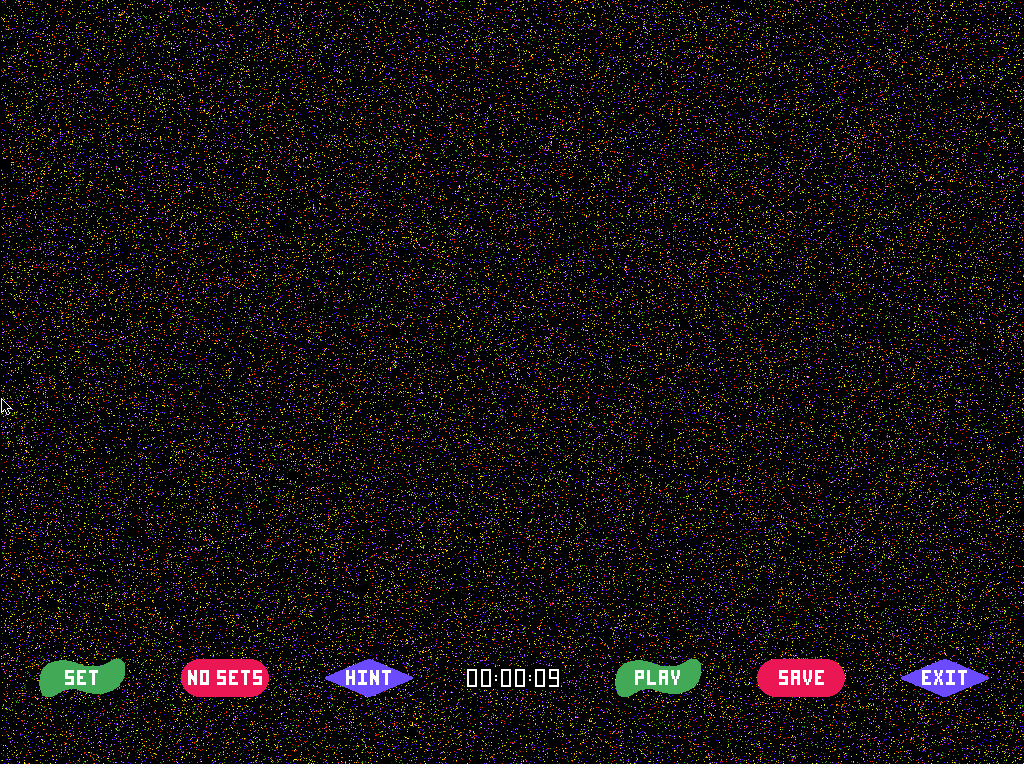
\includegraphics[scale=0.3]{game_pause.png}
\caption{A Paused game.}
\label{game_pause}
\end{center}
\end{figure}

If the player pauses the game, the timer is stopped and the cards are hidden. Also, the pause button is replaced with a play button. Although they are still shown, the Set, No Sets and Hint buttons have no effect. The pause screen can be observed in Figure~\ref{game_pause}.

\begin{figure}[htbp]
\begin{center}
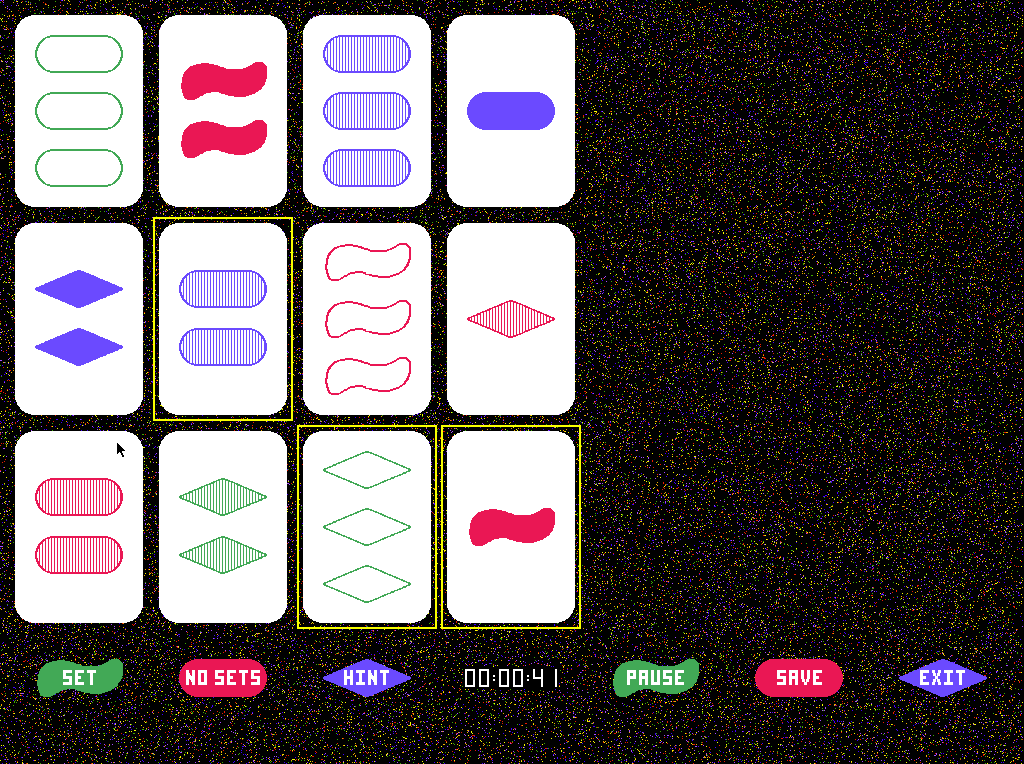
\includegraphics[scale=0.3]{game_select.png}
\caption{A Set selected.}
\label{game_select}
\end{center}
\end{figure}

In addition to selecting the buttons, the mouse is also used to select the cards. If the user clicks on a card, that card will be highlighted with a frame. Another click on the same card and the frame is removed. To form a set, the player must select 3 cards, as shown in Figure~\ref{game_select} and press the button Set.

\begin{figure}[htbp]
\begin{center}
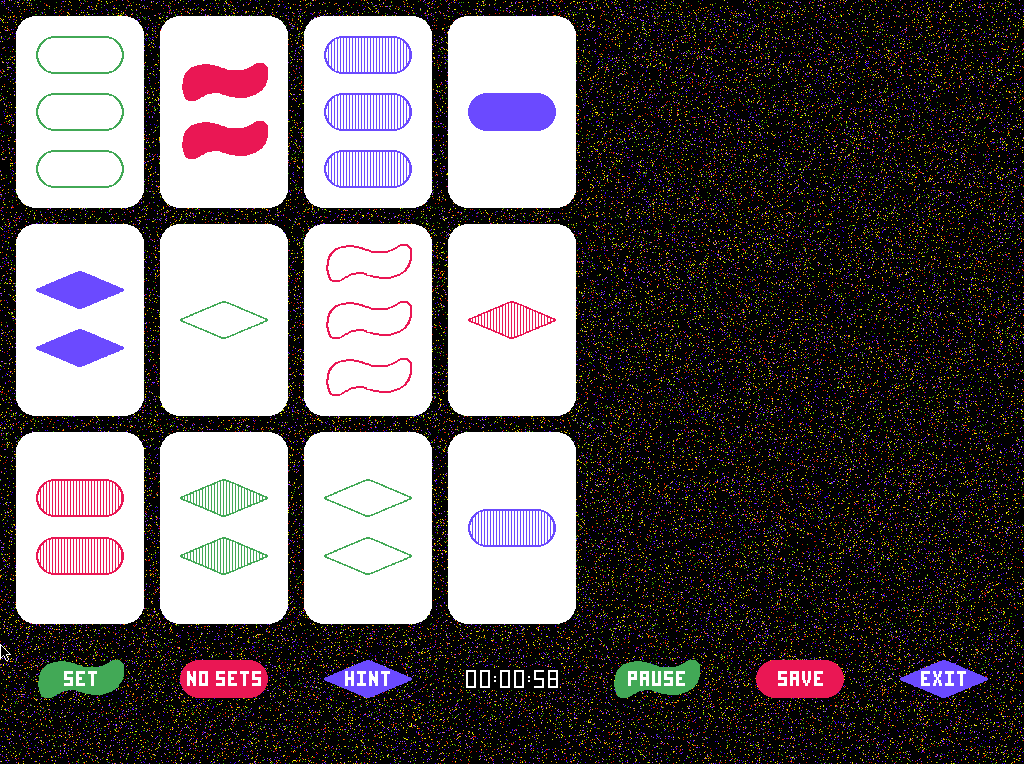
\includegraphics[scale=0.3]{game_add.png}
\caption{Three new cards.}
\label{game_add}
\end{center}
\end{figure}

After the Set button has been pressed, the 3 cards forming the set are removed and 3 new cards are added in their places, as can be seen in Figure~\ref{game_add}.

\begin{figure}[htbp]
\begin{center}
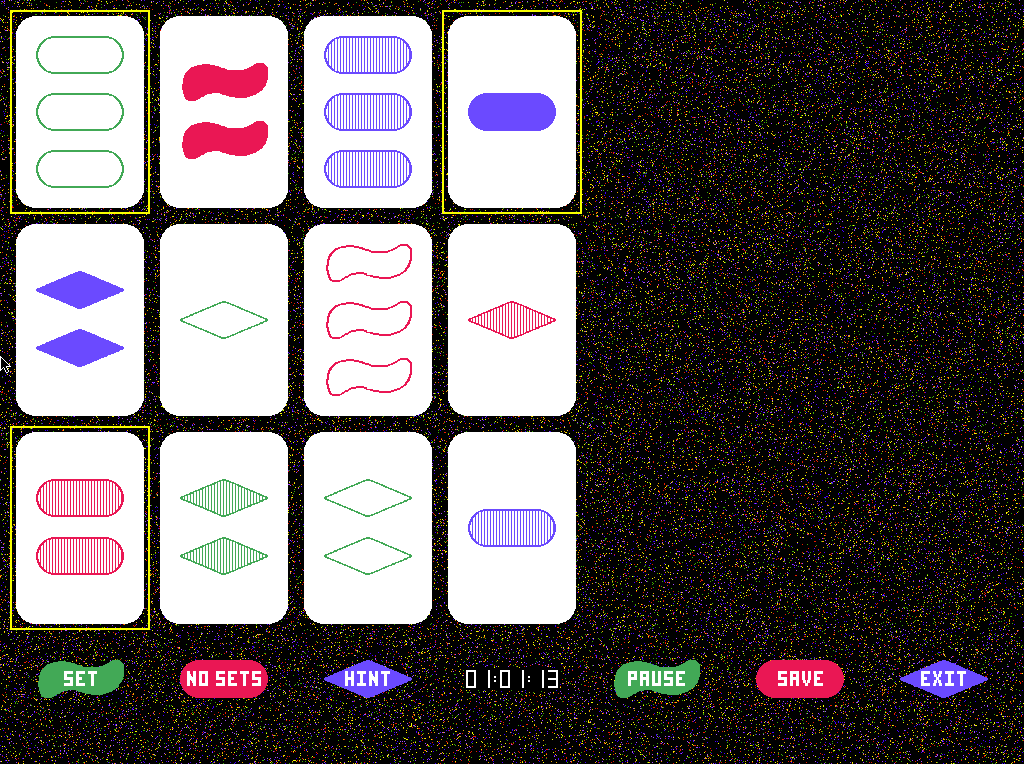
\includegraphics[scale=0.3]{game_hint.png}
\caption{Three hints to form a new Set.}
\label{game_hint}
\end{center}
\end{figure}

If the player asks for a hint, a new set card is selected. Unless there are no sets, in which case, three new cards are added forming a total of 15 cards in display. This can go up to 21 cards at most, since with that many cards there is always at least one set. Even 21 cards is a very rare event, having occurred only once in all our testing. For every hint, the player incurs in a time penalty of 20 minutes, unless there are no sets, in which case the penalty is 10 minutes. For example, if the player asks for all the three hints to form a set, the penalty will be 1 hour, as seen in Figure~\ref{game_hint}. There are also penalties for choosing the wrong set, 30 minutes, and for pressing the No Sets button when there are Sets in display, 20 minutes.

\begin{figure}[htbp]
\begin{center}
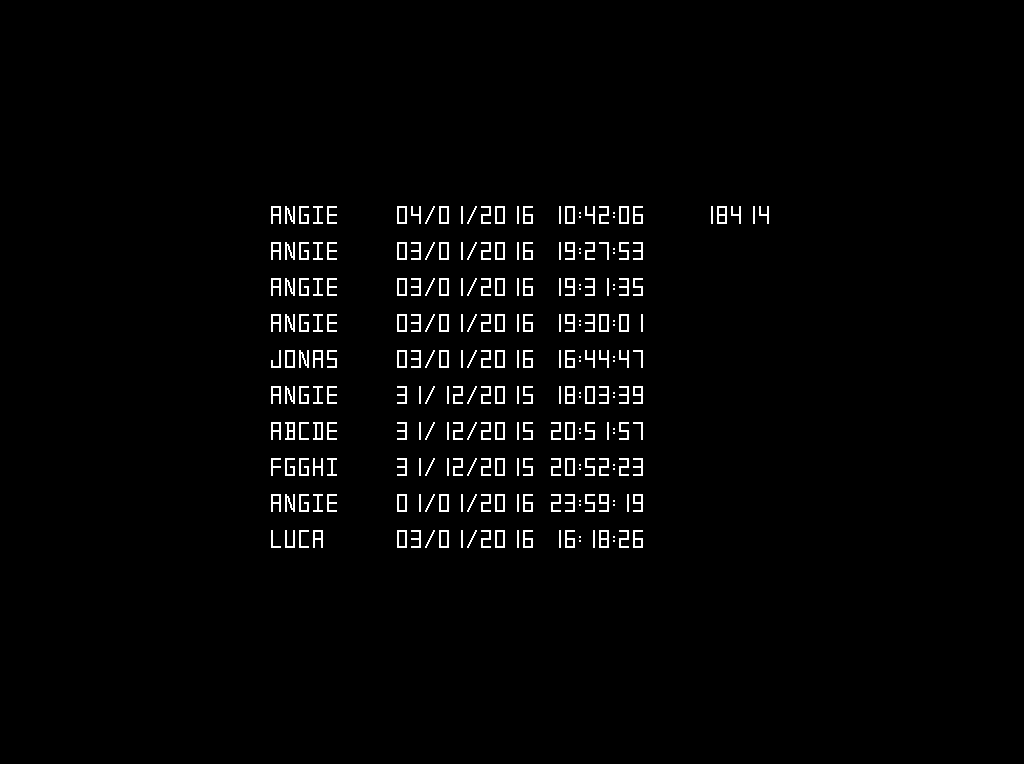
\includegraphics[scale=0.3]{game_score.png}
\caption{The game high scores.}
\label{game_score}
\end{center}
\end{figure}

At the end of a game, when there are no more sets, the new list of game high scores is presented, as shown in Figure~\ref{game_score}. At this time, pressing Esc will lead the player back to the initial menu, where they can choose to start a new game or simply leave the application by pressing Esc again.

\chapter{Project status}

As we saw above, not all intended game functionalities have been fully implemented. Indeed, the game modes for Hot Seat, Sudden Death and Two Player where not implemented. Also, the Load and Save Game features where not implemented. Since Two Player mode was the one intended to use the serial port, this device was not used and, as we will see, it was the only device that was not used.

Table~\ref{table} shows each device used.

\begin{center}
\begin{tabular}{ | c | l | c | }
	\hline
	Device 	&	What for	&	Int.	\\\hline
	Timer 	&	To keep track of the game time	&	Y	\\\hline
	Keyboard	&	To input player names and to choose game functionalities	&	Y	\\\hline
	Mouse	&	To select game cards, menu options and game buttons	&	Y	\\\hline
	Video card	&	To show the game menus, cards and other game objects	&	N		\\\hline
	RTC	&	To show the date and time in the log of high scores	&	N	\\\hline
\end{tabular}
\captionof{table}{Devices used}
\label{table}
\end{center}

\section{Timer}

In order to keep track of the game time, we used the Timer in interruption mode. For this purpose we used the functionality of Timer 0 that generates 60 interruptions for every second that passes. We used a Timer struct that keeps track of the number of interruptions since the last second, as well as the total time (hours, minutes and seconds) since the game started. When the game is paused, the timer interruptions are ignored. This happens when we are in the menus as well. Also, if a new game is started, the timer is reset back to 0.

We have specific files called timer to implement these functionalities. Also, in the file game.c, there are several uses of the timer functions. In lines 88-97, where we create a new timer for the game. In lines 417-457, where the time penalties are computed. In lines 470-482, where the timer interruptions are first handled, still being application independent. In lines 584-593, where the final game score is calculated. In lines 662-730, where the application dependent part of the timer interruptions is processed. In lines 733-831 where the timer interruptions are first subscribed and at the end unsubscribed.

\section{Keyboard}

The keyboard is used by the players as an alternative to pressing the buttons. Also, the Esc key is always used to exit to the initial menu, unless we are already in the initial menu, in which case it is used, to exit the game. In the game menus where name (or number) input is needed, the keyboard is also used for this effect and the Enter key allows the player to proceed.

All these keyboard features are implemented using interruptions. After each interruption the scan code generated is stored in the Keyboard struct. Only then, the application dependent interruption processing is done.

There are specific files called keyboard to implement all keyboard functionalities. Also, in the file game.c, these functions are called. In lines 71-78 where the game keyboard struct is created. In lines 146-164 where the button corresponding to each key is determined. In lines 470-482, where the keyboard interruptions are first handled, still being application independent. In lines 662-730, where the application dependent part of the keyboard interruptions is processed. In lines 733-831 where the keyboard interruptions are first subscribed and at the end unsubscribed.

Since the keyboard is also used in the menus, the file menu.c also implements keyboard functionalities. In lines 48-78 a keyboard digit (numbers 1 to 9) is attributed to the corresponding key. In lines 80-193 a keyboard letter is attributed to the corresponding key. In lines 312-351, where the application dependent part of the keyboard interruptions for the menus is processed. 

\section{Mouse}

The mouse is used throughout the menus two chose each option. Also, it is used to press buttons and select cards during gameplay. This is done with interruptions generated every time the mouse moves or a mouse button is pressed. We have created a Mouse structure to keep track of the mouse position on screen (so that it can be displayed) and store information about the buttons pressed.

There is a set of mouse files to implement the mouse struct and the functions that deal with it. Also, in the file game.c, there are several calls to the mouse functions. In lines 71-78 where the game mouse struct is created. In lines 166-201 where the button corresponding pressed by the mouse is determined. In lines 203-238 where the index of the card selected by the mouse is determined In lines 470-482, where the mouse interruptions are first handled, still being application independent. In lines 662-730, where the application dependent part of the mouse interruptions is processed. In lines 733-831 where the mouse interruptions are first subscribed and at the end unsubscribed.

Since the mouse is also used to navigate the menus, the file menu.c also implements mouse functionalities. In lines 195-242 several functions are implemented to determine the option chosen according to the game menu. In lines 244-287 the functionality corresponding to each button is called. In lines 312-351, the application dependent part of the mouse interruptions for the menus is processed. 

\section{Video card}

The video card is used to display all game objects. This is essentially done using xpm files for each image, letter or number that is displayed. In order to improve the performance of the game, we used double buffering, with the game objects being written to one of the game buffers and latter copied to the actual video memory. There are several buffers in use throughout the game. Each buffer has an intended type of object, for example, we have a mouse buffer, a timer buffer, a cards buffer, etc. This allows us to add or remove objects while keeping the background intact. 

Initially there was a specific background image to use during game play, and this image is still in the xpm files. But the final game version has a randomly generated background. Each pixel will be either black, red, green, blue, yellow, orange or purple. The probability of being black is 10 times higher than that of having another color, because black allows for better visualization. The use of a random background allows for some change, so that the same background all the time does not become tiresome.

The video mode we used is 0x105, which has a resolution of 1024 x 768 and a palette of 64 colors. We did not use moving objects or VBE functions to change the color palette. We did use fonts, by including xpm files with the letters and the numbers. The letters and numbers have a digital clock appearance, providing the game with a retro look.

There is a folder called images that contains all the game xpm files. Some of these files are organized into subfolders and their names are very clear to their content.

There are specific files for the graphics, the vbe files and the video\_gr files, where the functions that correspond only (or mostly) to the graphics card are implemented. Also, in the file game.c the graphics cards functions are used several times. In lines 64-70 where the game graphics struct is created. Throughout the whole file, whenever a card is added or removed or the mouse and timer need to be displayed, to draw the background, etc. These graphics are easy to recognize since they all start with vg\_. There is also a prolific use of graphics functions in the menu files, since they are needed there to draw the menus, the keyboard input and the mouse.

\section{RTC}

The RTC is used to obtain the date and time when a game is finished. This is then used in the high scores log, to keep track of when a certain high score was obtained. Thus we use only the reading date and time RTC functionalities, we do not use alarms or RTC interruptions.

There are specific files called rtc where the RTC structure and its functions are implemented. However, as usual, these functions are then called in the file game.c. In lines 98-108, where the game RTC structure is created. In lines 606-620 where the game is scored, after it is finished.

\chapter{Code organization/structure}

Since the whole project was done alone, there are no descriptions of the work distribution in this chapter. This reduces the importance of determining the weight of each module in the whole project. Basically the module game has the most weight, about 20\%. The other modules have more or less the same weight, with graphics being more than most and the rtc and the timer being less.

\section{Game module}

This is the main module of our application. It initializes the game structure and, within that, one structure for each game device. It also contains several functions for dealing with Set specific functionalities, like adding or removing cards. The interruption handlers, both initial and application dependent are also implemented here. Although the initial interruption handler simply calls the handler for each specific device, which is implemented in its own file. This file also contains the function run\_game, which calls all other functions recursively. It creates a new game, subscribes the necessary interruptions, begins an interruption loop and finishes everything by cleaning up.

This module contains two main structures. The game structure, that contains a pointer for each game device and for the game state structure. The game state structure, as the name implies, contains the current game state, with the number of cards dealt, the ones that are selected, the indicators to remove or add cards etc. The game state structure also contains an actual state in enumeration form, indicating if we are in play or pause, in a game menu, in game over or in scoring mode. 

\section{Logic module}

This module implements the game logic, it contains functions to decide if three given cards form a set or if there are no sets in display. There is also a function that looks for sets in the display, so that hints can be given. Although it is not a very extensive module, it is where the core of Set really lies. We think that the way to determine wether three given cards form a set is clever. In any case, other modules where more difficult to implement, since dealing with the idiosyncrasies of each device presented several problems.

\section{Dispatcher module}

The dispatcher has a generic function for subscribing interruptions as well as a generic interruption loop function. The latter function has two function pointers as arguments, one for initial interrupt handling and another for application dependent interruption handling.

\section{Menu module}

This module contains the game menu functionalities. It implements a Menu structure, which contains a menu state, indicating the current menu (initial, new game, single player, etc), and also the number of players, the player names and the game mode chosen. While the game is in menu mode, this module is in control, later giving control back to the game module, for the game play.

\section{Images and XPM modules}

The images module contains a few functions to obtain the xpm pointers so that each game object can be displayed. There is also a file called read\_xpm.c where the xpm files are processed. This last module was provided by the Professor and was not coded by me, but by Professor João Cardoso.

\section{High score module}

This module implements the Highscore structure, where a game high score is stored. This contains a player name, an actual score and a pointer to a DateTime structure which contains the date and time when the high score was obtained. A game structure contains an array with 10 Highscore structures, since that is the number of high scores kept in log. The module also implements functions to read the high scores from a file and save them at the end of a game. There is also a function to determine the position of a new score withing the high scores array.

\section{Timer, Keyboard, Mouse and RTC modules}

Although these modules are completely independent we describe them together since they have been mentioned in the previous chapter. Each one contains a structure for the respective device as well as the necessary functions to deal with that device. Many of these are low level functions that actually interface with the device controller registers.

\section{VBE and video graphics modules}

The VBE module implements the VBE standard functions. This is the actual module that interfaces with the video graphics device. The structures in this module where provided by Professor Pedro Souto, but most of the functions where coded by me, as instructed in class. The video graphics module, whose name is video\_gr, implements many functions that draw the actual game objects, such as the background, the cards, the menus, the mouse and the time. There is also a graphics structure in this file, that contains the pointers to the cards, letters and numbers xpm's, the several buffers for cards, background, mouse, etc and the video memory pointer.

\section{Function call graph}

\begin{figure}[htbp]
\begin{center}
\includegraphics[scale=0.4]{function.png}
\caption{The function call graph for run\_game.}
\label{function}
\end{center}
\end{figure}

The function call graph for run\_game can be observed in Figure~\ref{function}. As stated above, run\_game is the main game function. It starts by creating a new game struct, then it subscribes the several interruptions (keyboard, mouse and timer) and starts the interruption loop with its two handlers, the interruption handler and the application handler, once the interruption loop is finished a destroy\_game function is called. 

The create game function itself calls several other create functions, since the game structure contains pointers to every device structure as well as menu, game state and highscore structures. The same applies to the destroy game function which calls several other destroyers. 

The application independent interruption handler calls for each specific interruption the corresponding handler, timer\_int\_handler, keyboard\_int\_handler and mouse\_int\_handler. 

The application dependent interruption handler will call the menu interruption handler if the game state indicates that we are in a menu. This menu handler has been described above, in addition to taking the appropriate action according to the mouse or keyboard inputs, it draws each specific menu as evidenced at the top right corner of the function call diagram.

Otherwise, during game play, it will, depending on the specific interruption, determine the selected card or button, check if the game state is correct, undo eventual card selections if necessary, take action on the final game state and draw the mouse and timer again. The state\_check function is used to check the player inputs according to the game logic, the player may denote as a Set something that is not, for example. The state\_undo functions is used to deselect a previously selected card if the player clicks the same card twice. Finally, the state\_action function takes into account the current game state and makes the necessary changes, like removing a Set of cards and adding new ones. These functions continuously invoke drawing functions for the mouse and the timer, because the mouse keeps moving and the game time keeps increasing.

At the end of the game, the interruption handler calls the score function, to compute the current game score, update the high scores, display them and save them. Then everything starts again, with the game going back to the initial menu and everything being reset.

Another function that is frequently called is copy\_buffer, which as the name suggests, copies a buffer with certain graphics to another buffer. This is used because of our double buffering, since we want to copy certain buffers to the video memory, for example.

\chapter{Implementation details}

The interruption handling was talked about frequently throughout the course, with its difficulty increasing and new features being added. Early on, we developed a generic method for interruption subscription and interrupt loop generation. These functions evolved with each lab and are at their finest in the final project. Indeed, now they make use of state machines, separate the application independent from the application dependent interruption handling and to the best of our knowledge are completely generic allowing any kind of interruptions to be subscribed and handled.

The use of state machines was encouraged in an earlier lab, but we only got around to it in the project. In the end they were probably the most useful feature we used, after the interruption handling functions. In addition to enumeration types for several component states, we used flags or indicators for certain events, as well as data fields to store important information. We consider these fields a part of our state machines, although they can also be viewed as another part of a larger structure that contains a state machine. We are quite please with our final state machines and the simplicity they provide for event handling.

Of course all of this makes use of the object orientation data structures. Although C is not an object oriented language, we believe the use of structs allows for a better code layering as well as some isolation of features. We made extensive use of structures, with at least one per module, in order to keep the code better organized and each data field stored in its proper place.

The whole project was conceived in layers from the start, with many modules being included from the very beginning. Even after that, each new device brought its own module and maybe some more. But, as usual, the haste in coding and seeing results led to earlier versions of the project having an extremely large game.c file with many different functionalities mixed. Later on, some code refactoring led to some of these functionalities being placed in previously created modules, while others led to the appearance of complete new modules. The main idea was to create a module for each structure and the functions that deal with it. This made further developments that much faster, since it was easier to find each specific function. 

Although not extensively, we used some debug methods that were studied. Much of the debugging was visual, since the graphics component was the first to be implemented. But there is also some printing debugs, that can be activated through the use of DEBUG constants.

In the final project version we did not use assembly code. The only function we could use assembly on was the keyboard, to get each scan code. But since it was not worth a better grader, we used the C version of that function instead.

We did not implement the UART and the use of the RTC was very straightforward, we simply check its registers, making sure it is not updating before, to get the current date and time.

\chapter{Conclusions}

Although Computer Laboratory is a difficulty course, perhaps the most difficult up to this point, and the work load is incredibly large, I found it most enjoyable. Perhaps the initial scare made me work harder and therefore learn more, but with a couple of exceptions concerning Math courses that were particularly attuned to my preferences, this was probably the most successful course I have ever taken.

The main useful suggestion I have is about the lab notes. I believe they should be all inclusive, instead of forcing the student to check the class notes, because that creates a time consuming back and forth. Also, in this year's lab notes, with the new method of having different pages per section, I think there should be a button to return to the course home page.

In terms of course organization, I find the nonexistence of practical lessons to deal with the serial port (and even the RTC) to be the worst part of the course. The serial port in particular is a very difficult subject for the student to do home alone. But quite frankly I do not have a better suggestion for it, because I do not think it wise to remove time from other classes. Perhaps at the beginning of the course, the setup should be done at home so that the first lab (video graphics in text mode) is finished in the first class. Or maybe some functions can be left as optional implementations (like the keyboard leds) so that some labs take one and a half classes instead of two.

I also think it would be useful for the students to have detailed feedback of what they should improve. Perhaps this could be done in some of the practical lessons. The general feeling is that even though some pointers were given, I probably have been making some of the same mistakes all along, which contradicts the principle that one should evolve while taking a course.

Another problem related to this is the fact the doubt clarification in the practical lessons was a very slow process. Honestly I think the teachers and students that are providing support could have done a better job of dividing their attention. Some groups where clear attention grabbers and in a room full of students it is not fair for the teacher to spend a quarter of class with the same group, while others are waiting. This is especially difficult in classes where delivery is right at the end. Perhaps a few more hours or a day should be given, so that the students may look for help outside of the class.

Regarding the project and my general performance, I was very pleased with the results throughout the semester, but would like to have done a lot more in the project. Even more than implementing the serial port, I would like to have finished the other game modes, as well as the save and load functionalities. Unfortunately, time was not on my side, as other courses demanded my attention. That said, I am very likely to finish this project at a later time, since Set is a game I like to play with my friends.

\end{document}
